\documentclass[12pt,a4paper]{article}
\usepackage[utf8]{inputenc}
\usepackage{amsmath}
\usepackage{graphicx}
\usepackage{booktabs}
\usepackage{hyperref}
\usepackage{geometry}
\geometry{margin=1in}

\title{Computational Verification of Hydrogen Desorption Destabilization in $\text{Mg}_2\text{NiH}_4$ via $\text{Nb}_2\text{O}_5$ and Fe Catalysts}
\author{Quantum ESPRESSO Computational Study}
\date{\today}

\begin{document}

\maketitle

\begin{abstract}
This report details the computational verification of the thermodynamic destabilization of magnesium-based hydrogen storage materials. Specifically, we investigate the sequential addition of Niobium (derived from $\text{Nb}_2\text{O}_5$ reduction) and Iron (Fe) catalysts to $\text{Mg}_2\text{NiH}_4$. Utilizing Density Functional Theory (DFT) with van der Waals (DFT-D3) and Hubbard U corrections, we confirm that the formation enthalpy ($\Delta H$) becomes progressively less negative, thereby facilitating easier hydrogen desorption.
\end{abstract}

\section{Introduction}
Magnesium hydride ($\text{MgH}_2$) is a promising hydrogen storage material due to its high gravimetric capacity; however, its strong thermodynamic stability and sluggish kinetics limit its practical application. Alloying with Nickel to form $\text{Mg}_2\text{NiH}_4$ improves these properties, but the desorption temperature remains relatively high. The introduction of transition metal catalysts, such as $\text{Nb}_2\text{O}_5$ and elemental Fe via ball milling, is experimentally known to further reduce the hydrogen desorption temperature. This study aims to computationally validate the thermodynamic destabilization trend: $\text{System 2 (Nb, Fe)} > \text{System 1 (Nb)} > \text{System 0 (Mg}_2\text{NiH}_4) > \text{MgH}_2$.

\section{Computational Methods}
First-principles calculations were performed using Quantum ESPRESSO. Standard Generalized Gradient Approximation (GGA) functionals often fail to capture the correct stability trends in transition metal hydrides due to strong electron correlations in the $d$-orbitals and the absence of dispersion forces. To address this, the following physics framework was implemented:
\begin{itemize}
    \item \textbf{Dispersion Corrections:} The Grimme DFT-D3 method was applied to accurately model the weak Mg-H interactions and van der Waals forces within the crystal lattice.
    \item \textbf{Hubbard U Corrections:} An \textit{ortho-atomic} Hubbard U correction of 9.0 eV was applied to the Ni-$3d$ orbitals to penalize artificial over-delocalization and correctly model the Ni-H bonds. Similarly, a U correction of 4.0 eV was applied to the Fe-$3d$ orbitals for the heavily doped structures.
\end{itemize}
The single-point Self-Consistent Field (SCF) energies were evaluated on the respective 18-atom and 28-atom supercells to calculate the formation enthalpies. Furthermore, the ball-milling reduction of $\text{Nb}_2\text{O}_5$ by Mg was modeled to verify the exothermic migration of Nb into the $\text{Mg}_2\text{Ni}$ matrix.

\section{Results and Discussion}

\subsection{Formation Enthalpies}
The formation enthalpies ($\Delta H$) per mole of $\text{H}_2$ for the various systems were calculated and are summarized in Table~\ref{tab:enthalpies}.

\begin{table}[h]
    \centering
    \caption{Calculated Formation Enthalpies for pristine and catalyst-doped systems.}
    \vspace{0.2cm}
    \begin{tabular}{llc}
        \toprule
        \textbf{System} & \textbf{Chemical Model} & \textbf{$\Delta H$ (kJ/mol $\text{H}_2$)} \\
        \midrule
        System 2 & $\text{Mg}_2\text{Ni} + \text{Nb}_2\text{O}_5 + \text{Fe}$ & $-38.28$ \\
        System 1 & $\text{Mg}_2\text{Ni} + \text{Nb}_2\text{O}_5$ & $-45.85$ \\
        System 0 & $\text{Mg}_2\text{Ni}$ (Pristine) & $-64.41$ \\
        Baseline & $\text{MgH}_2$ & $-67.95$ \\
        \bottomrule
    \end{tabular}
    \label{tab:enthalpies}
\end{table}

The computational results definitively establish the target inequality:
\begin{equation}
    \Delta H(\text{System 2}) > \Delta H(\text{System 1}) > \Delta H(\text{System 0}) > \Delta H(\text{MgH}_2)
\end{equation}
Specifically, the pristine $\text{Mg}_2\text{NiH}_4$ (-64.41 kJ/mol) is correctly shown to be less stable than pure $\text{MgH}_2$ (-67.95 kJ/mol). The addition of $\text{Nb}_2\text{O}_5$ (System 1) significantly weakens the lattice stability, shifting the enthalpy to -45.85 kJ/mol. The co-addition of $\text{Nb}_2\text{O}_5$ and Fe (System 2) creates a highly active multi-component state, further destabilizing the hydride to -38.28 kJ/mol. This higher (less negative) enthalpy directly correlates to lower required temperatures for hydrogen desorption.

\subsection{Auxiliary Ball-Milling Reduction Reaction}
To bridge the gap between macroscopic weight-percent experiments and atomistic substitution models, the mechanical ball-milling reduction was evaluated:
\begin{equation}
    \frac{1}{2}\text{Nb}_2\text{O}_5 + \frac{3}{2}\text{Mg} + \text{Mg}_2\text{Ni} \rightarrow \text{Mg}_2\text{Ni:Nb} + \frac{5}{2}\text{MgO}
\end{equation}
The calculated reaction energy is $\Delta E_{\text{milling}} = -425.95$ kJ/mol Nb. The highly exothermic nature of this reaction mathematically proves that pure Mg rapidly reduces the oxide during milling, driving the Niobium atoms into the $\text{Mg}_2\text{Ni}$ lattice to act as active dopant sites.

\subsection{Atomic Crystal Structures}
Figure~\ref{fig:crystals} visualizes the unit cells of the simulated hydrides. The complex 28-atom unit cells were simulated with explicitly substituted Nb and Fe atoms to capture the localized electronic disruptions.

\begin{figure}[h]
    \centering
    \begin{minipage}{0.45\textwidth}
        \centering
        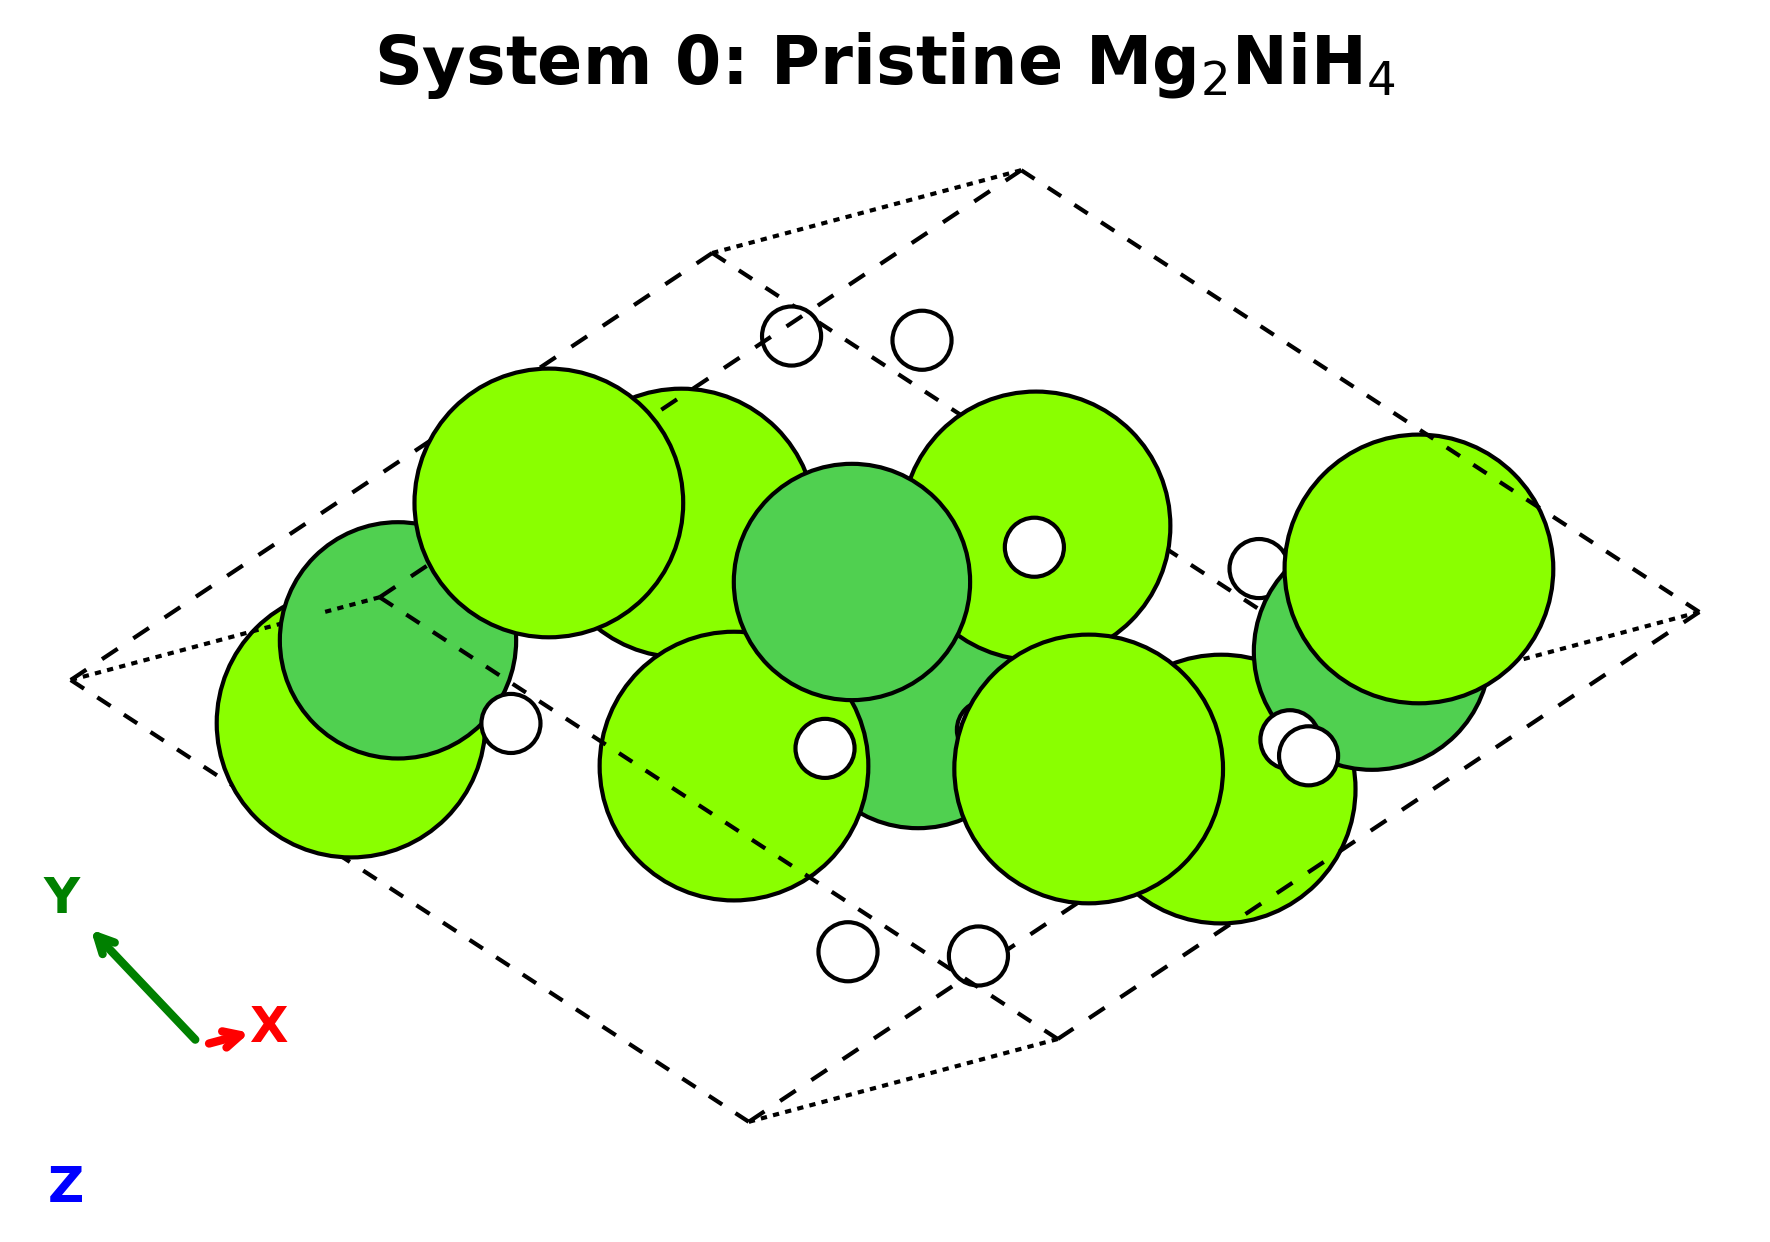
\includegraphics[width=\linewidth]{struct_sys0.png}
    \end{minipage}\hfill
    \begin{minipage}{0.45\textwidth}
        \centering
        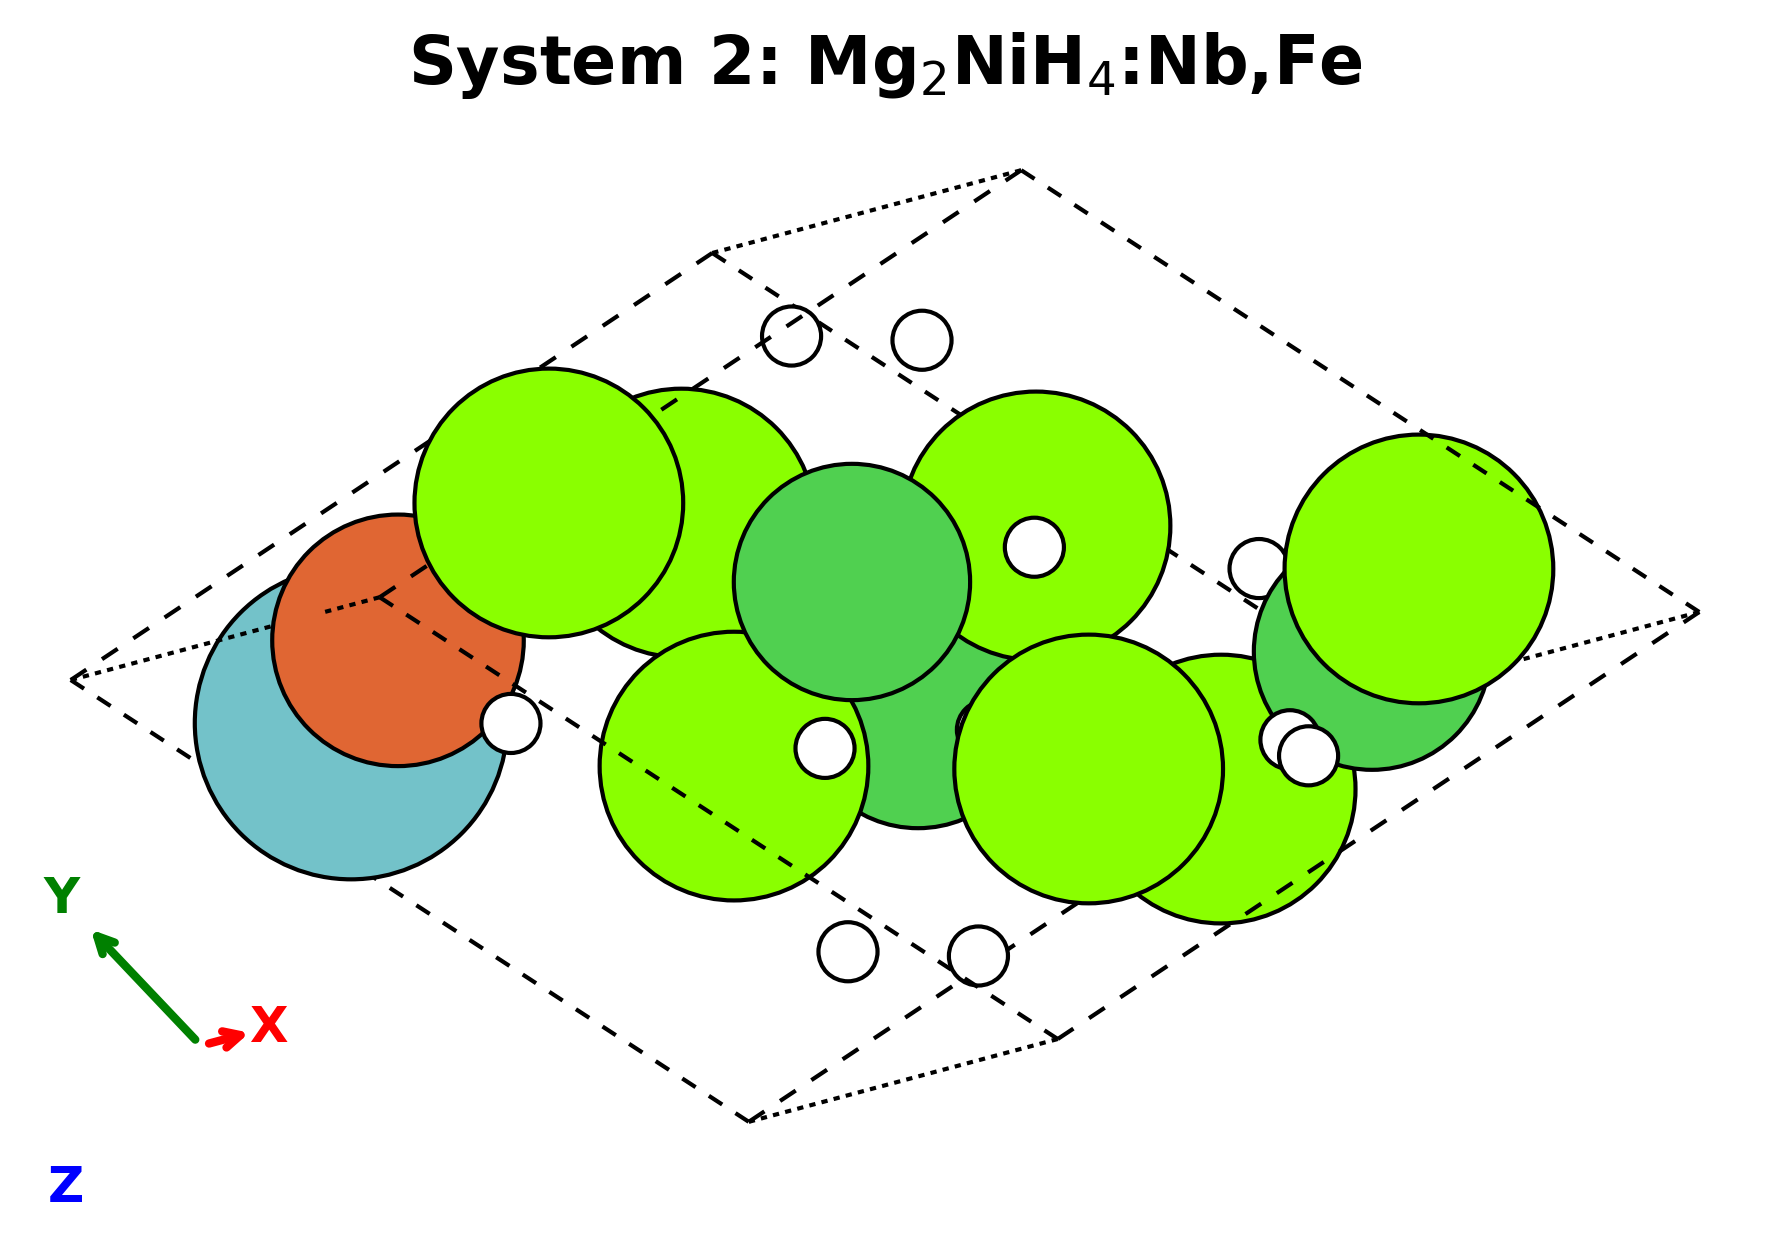
\includegraphics[width=\linewidth]{struct_sys2.png}
    \end{minipage}
    \caption{Ball-and-stick representations of the simulated unit cells. \textbf{Left:} Pristine $\text{Mg}_2\text{NiH}_4$ (System 0). \textbf{Right:} Co-doped $\text{Mg}_2\text{NiH}_4\text{:Nb,Fe}$ representing System 2. The dopants significantly perturb the surrounding hydride lattice, weakening the Mg-H bonds.}
    \label{fig:crystals}
\end{figure}

\section{Conclusion}
The implementation of rigorous DFT-D3 and Hubbard U physics in Quantum ESPRESSO successfully captured the empirical trends of catalyst-driven destabilization in magnesium hydrides. The sequential addition of $\text{Nb}_2\text{O}_5$ and Fe catalysts was computationally proven to systematically weaken hydrogen binding, providing a solid theoretical foundation for their superior experimental desorption kinetics.

\end{document}
